\documentclass[11pt]{article}
\usepackage{times,float, multicol}
\usepackage[pdftex]{graphicx}
\usepackage[rflt]{floatflt}
\usepackage{hyperref}


\setlength{\textwidth}{6.5in}
\setlength{\textheight}{9.0in}
\setlength{\topmargin}{-.5in}
\setlength{\oddsidemargin}{-.0600in}
\setlength{\evensidemargin}{.0625in}

\newcommand{\secref}[1]{Section~\ref{#1}}

\newcommand{\doublespace}{\baselineskip0.34truein}
\newcommand{\singlespace}{\baselineskip0.16truein}
\newcommand{\midspace}{\baselineskip0.24truein}
\newcommand{\midplusspace}{\baselineskip0.26truein}

\def\TreeSearch{{TreeSearch}}

\title{{\TreeSearch} User Guide\\ {\large Version 0.9}}

\author{Derrick Stolee \\ 
	University of Nebraska-Lincoln\\ 
	\texttt{s-dstolee1@math.unl.edu}
       }
       
\begin{document}

\maketitle
\vspace{-.3in}
\begin{abstract}
	The {\TreeSearch} library abstracts the structure of a search tree
		in order to manage jobs in a distributed computation.
	This document details the strategy of {\TreeSearch} along with
		implementation, compilation, and execution details.
	An example application is also given.
\end{abstract}

\section{Introduction}
\label{sec:Introduction}

The computation path of a dynamic search frequently takes the form of a rooted tree.
One important property of each node in this tree is that the computation at that
	node depends only on the previous nodes in the ancestral path leading
	to the root of the computation.
If the search is implemented in the usual way, subtrees operate independently.

For a search of this type, all search nodes at a given depth 
	can be generated by iterating through the search tree, but 
	backtracking once the target depth is reached.
Each of the subtrees at this depth can be run independently,
	and hence it is common to run these jobs concurrently 
	(See \cite{ClassificationAlgorithms} Chapter 5 for more information).

The {\TreeSearch} library was built to maximize code reuse for these types of search.
It abstracts the structure of the tree and the recursive nature of the search into
	custom components available for implementation by the user.
Then, the ability to generate a list of jobs, run individual jobs, and submit the list
	of jobs to a cluster are available with minimal extra work.
	
{\TreeSearch} is intended for execution 
	on a distributed machine using
	Condor \cite{condor-practice},
	a job scheduler that uses idle nodes of a cluster or network.
Condor was chosen as its original development was meant for
	installation in computer labs and office machines 
	at the University of Wisconsin--Madison
	to utilize idle computers.
	
The C++ portion of {\TreeSearch} 
	is independent of Condor.
The Python scripts which manage the input and output files
	as well as modifying the submission script are
	tied to Condor, but 
	could be adapted for use in other schedulers.


\subsection{Acquiring \TreeSearch}

The latest version of {\TreeSearch} and its documentation
	is publicly available on GitHub \cite{github} at the address
	\href{http://www.github.com/derrickstolee/TreeSearch/}{http://www.github.com/derrickstolee/TreeSearch/}.


\section{Strategy}
\label{sec:Strategy}

Let us begin by describing the general structure and process of an abstract
	tree-based search.
There is a unique root node at depth zero.
Each node in the tree searches in a depth-first, recursive manner.
There are a number of children to select at each node.
One may select this child through iteration or selecting via a numerical order.
Before searching below the child, a pruning procedure may be called to attempt to 
	rule out the possibility of a solution below that child.
Another procedure may be used to find if this node is a solution.
Now, the search recurses at this node until its children are exhausted 
	and the search continues back to its parent.
%The tree search process, what order are things called?

\subsection{Subtrees as Jobs}

%Talk about the job descriptions.
This tree structure allows for search nodes to be described via the 
	list of children taken at each node.
Typically, the breadth of the search will be small and these descriptions take very little space.
This allows for a method of describing a search node independently of 
	what data is actually stored by the specific search application.
Moreover, the application may require visiting the ancestor search nodes in order
	to have consistent data.
With the assumption that each subtree is computationally independent of other subtrees at the same level,
	one can run each subtree in a different process in order to achieve parallelization.
These path descriptions make up the input for the specific processes in this scheme.

\begin{floatingfigure}{3in}\centering
	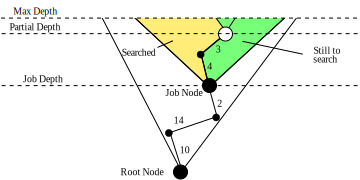
\includegraphics[width=3in]{figures/Jobs}
	\caption{\label{fig:jobs}A partial job description.}
\end{floatingfigure}


Each path to a search node qualifies as a single job, where the goal 
	is to expand the entire search tree below that node.
A collection of nodes where no pair are in an ancestor-descendant relationship 
	qualifies as a list of independent jobs.
Recognizing that the amount of computation required to expand 
	the subtree at a node is not always a uniform value,
	{\TreeSearch} allows a maximum amount of time 
	within a given job.
In order to recover the state of the search when the execution times out,
	the concept of \emph{partial jobs} was defined.
A partial job describes the path from the root to the current search node.
In addition, it describes which node in this path is the original job node.
The goal of a partial job is to expand the remaining nodes in the
	subtree of the job node, without expanding any nodes to 
	the left of the last  node in this path.
See Figure \ref{fig:jobs} to an example partial job and its position in the
	job subtree.

\subsection{Job Descriptions}

% How jobs/partials/solutions/completes/statistics are represented in the output

The descriptions of jobs and partial jobs are described using text files
	in order to minimize the I/O constraints on the distributed system.
The first is the standard job, given by a line starting with the letter \texttt{J}.
Following this letter are a sequence of numbers in hexadecimal.
The first two should be the same, corresponding to the depth of the node.
The remaining numbers correspond to the child values at each depth from the root to the job node.

A partial job is described by the letter \texttt{P}.
Here, the format is the same as a standard job except the first number describes the depth of the job node
	and the second number corresponds to 
	the depth of the current node.
For example, the job and partial job given in Figure \ref{fig:jobs} are described by the strings below:

\begin{verbatim}
    J 3 3 10 14 2
    P 3 5 10 14 2 4 3
\end{verbatim}

\subsection{Customization}

The {\TreeSearch} library consists of an iterative implementation of the abstract search.
The corresponding actions for a specific application are contacted via extending 
	the \texttt{SearchManager} class and implementing certain virtual functions.
The list of functions available are given in Table \ref{tbl:functions}.

	
\begin{table}[htb]\centering
\begin{tabular}[H]{|ll|p{3in}|}
	\hline
	\texttt{LONG\_T} & \texttt{pushNext()} & 
		Deepen the search to the next child of the current node.\\
	\hline
	\texttt{LONG\_T} & \texttt{pushTo(LONG\_T child)} & 
		Deepen the search to the specified child of the current node.\\
	\hline
	\texttt{LONG\_T} & \texttt{pop()} & 
		Remove the current node and move up the tree.\\
	\hline
	\texttt{int} & \texttt{prune()}  & 
		Perform a check to see if this node should be pruned.\\
	\hline
	\texttt{int} & \texttt{isSolution()} & 
		Perform a check to see if a solution exists at this point.\\
	\hline
	\texttt{char*} & \texttt{writeSolution()} & 
		Create a buffer that contains a description of the solution.\\
	\hline
	\texttt{char*} & \texttt{writeStatistics()}  & 
		Create a buffer that contains custom statistics.\\
	\hline
\end{tabular}
\caption{\label{tbl:functions}List of virtual functions in the \texttt{SearchManager} class.}
\end{table}


In addition to supplying the logic behind these functions, 
	protected members of the \texttt{SearchManager} class can be modified to change the
	operation of the search.
These parameters are listed in Table \ref{tbl:members}.

	
\begin{table}[htb]\centering
	\small
\begin{tabular}[H]{|lll|p{2.5in}|}
	\hline
	Type & Name & Option & Description\\
	\hline
	\texttt{int} & \texttt{maxdepth} & \texttt{-m [N]} &
		The maximum depth the search will go.  
		In generate mode, a job will be output with
		job description given by the current node. \\
	\hline
	\texttt{int} & \texttt{killtime} & \texttt{-k [N]} &
		Number of seconds before the search is halted.  
		If the search has not halted naturally, a partial job is output at the current node.\\
	\hline
	\texttt{int} & \texttt{maxSolutions} & \texttt{--maxsols [N]} &
		The maximum number of solutions to output.  
		When this number of solutions is reached, a partial job is output and the search halts.\\
	\hline
	\texttt{int} & \texttt{maxJobs} & \texttt{--maxjobs [N]} &
		The maximum number of jobs to output (generate mode).  
		When this number of jobs is reached, a partial job is output and the search halts.\\
	\hline
	\texttt{bool} & \texttt{haltAtSolutions} & \texttt{--haltatsols [yes/no]} &
	If \texttt{true}, the search will stop deepening if \texttt{isSolution()} signals a solution. 
	If \texttt{false}, the search will continue until specified by \texttt{prune()} or \texttt{maxdepth}.\\
	\hline
\end{tabular}
\caption{\label{tbl:members}List of members in the \texttt{SearchManager} class.}
\end{table}



\section{Integration with \TreeSearch}
\label{sec:Integration}

This section details the specific interfaces for
	implementation with {\TreeSearch}.

It is important to understand the order of events
	when the search is executing.
The search begins when the \texttt{doSearch()} methd
	is called.
The first call initializes the search, including
	starting the kill timer.
Then, each recursive call expands the current search node
	at the top of the stack.
Figure \ref{fig:doSearch} describes the actions
	taken by the recursive \texttt{doSearch()} 
	method takes at each search node.
	
	
\begin{figure}[h]
	\centering
	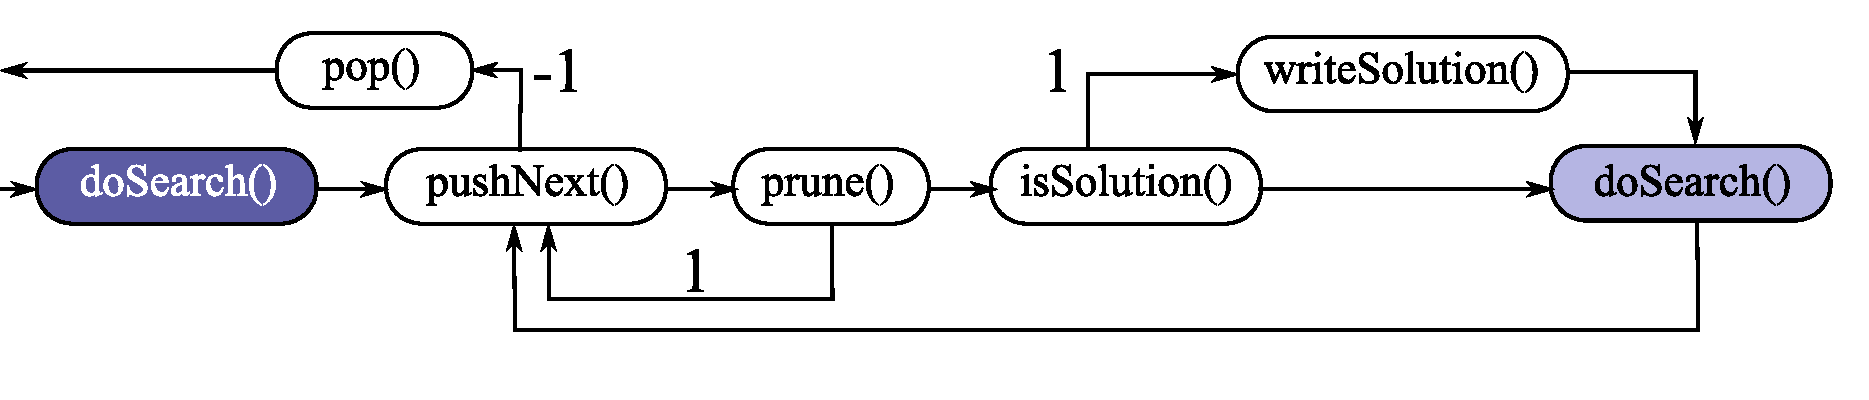
\includegraphics[width=0.9\textwidth]{figures/conceptFlowchart}
	\caption{\label{fig:doSearchSmall}The conceptual operation of the \texttt{doSearch()} method.}
\end{figure}
	
\begin{figure}[p]
	\centering
	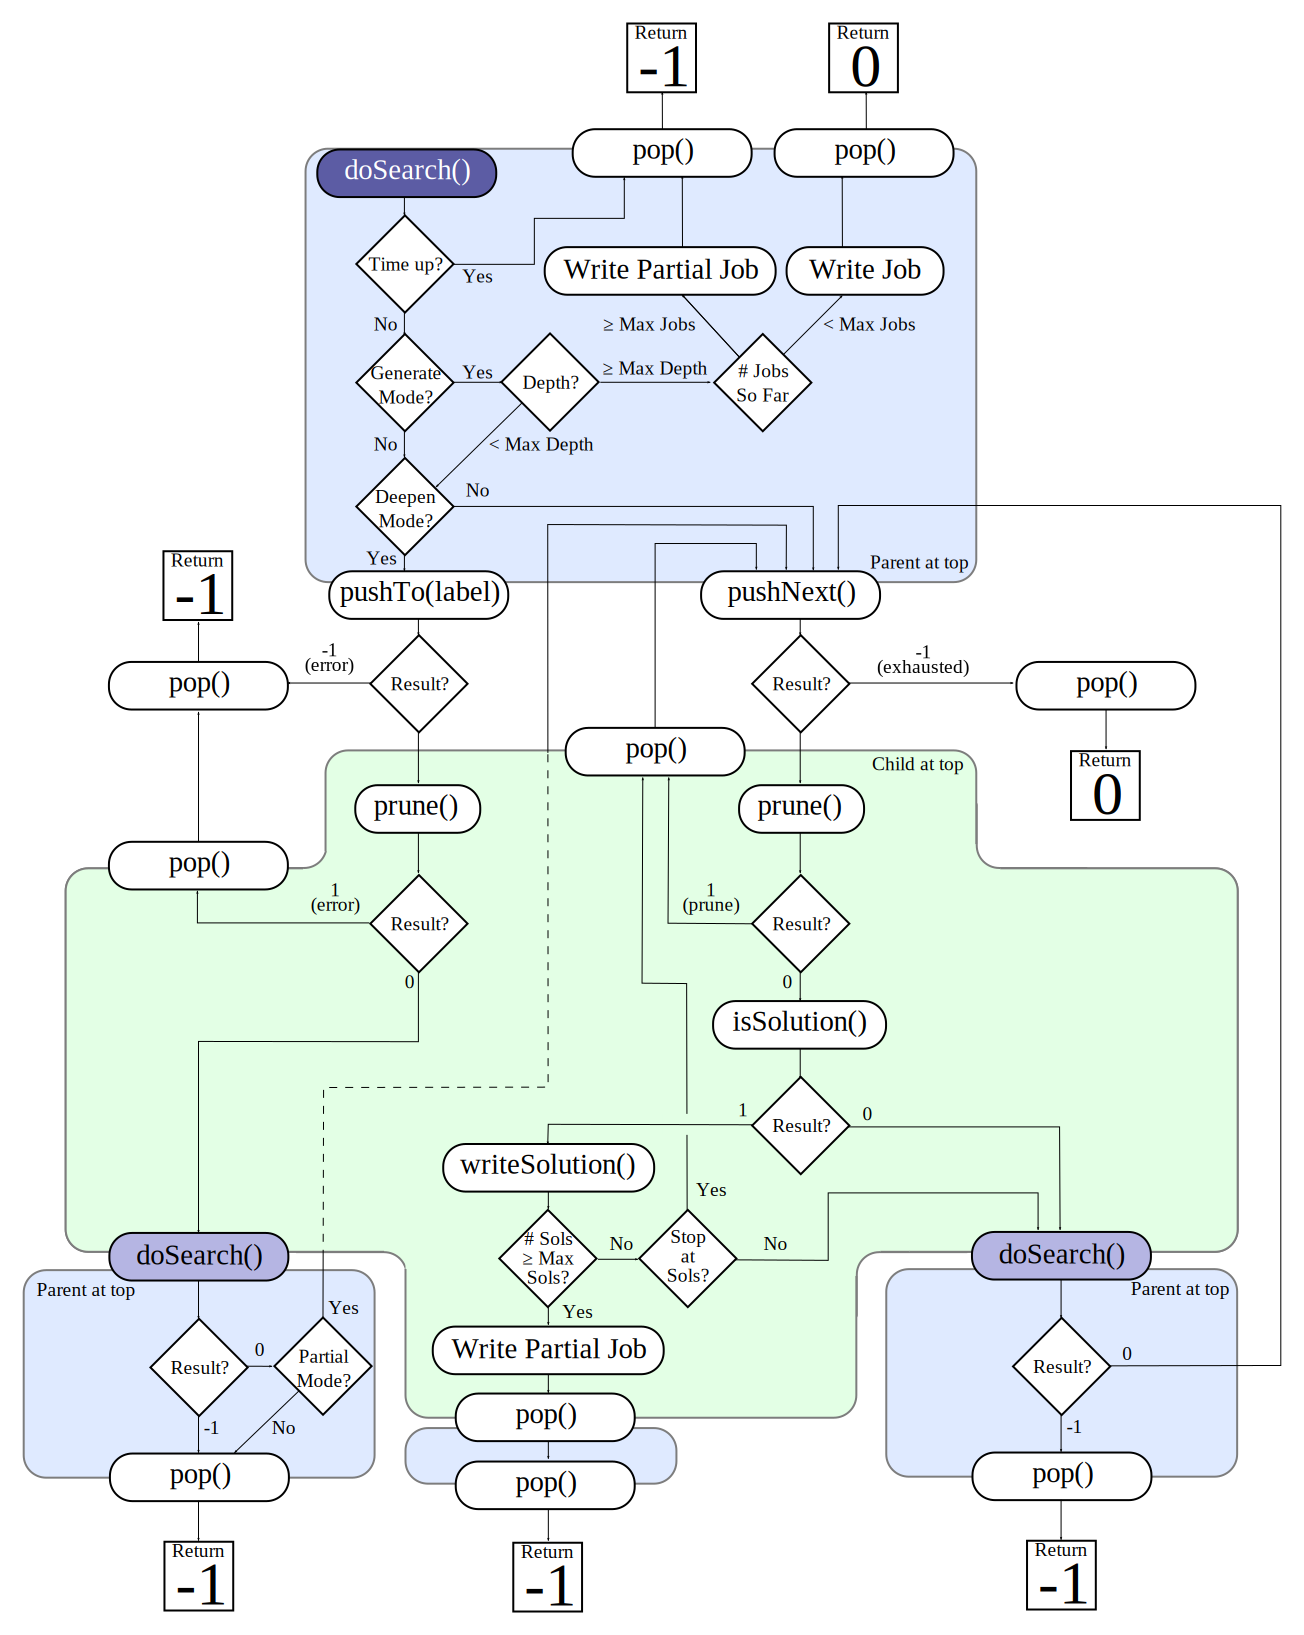
\includegraphics[height=0.95\textheight]{figures/doSearchFlowchart}
	\caption{\label{fig:doSearch}The full operation of the \texttt{doSearch()} method.}
\end{figure}

\subsection{Virtual Functions}

The two most important methods are the
	\texttt{pushNext()} and \texttt{pushTo(LONG\_T child)} methods.
Both deepen the search, 
	manage the stack, 
	and control the job descriptions.
Each returns a child description (of type \texttt{LONG\_T})
	
\noindent{\bf \texttt{pushNext()}:}
	Advance the search stack using the next augmentation available at the current node.
	Return a label of \texttt{LONG\_T} type which describes the augmentation.
	Return $-1$ if there are no more augmentations to attempt at this stage,
		signaling a \texttt{pop()} operation.
	
\noindent{\bf \texttt{pushTo(LONG\_T child)}:}
	Advance the search stack using the augmentation specified by \texttt{child}.
	If the augmentation fails as specified, return $-1$, and the search will terminate in error.
	{\bf Note:} If this method is called during the partial portion of a job description,
		the later augmentations will be called using the \texttt{pushNext()} method,
		so the current augmentation must be stored for later.
	
\noindent{\bf \texttt{pop()}:}
	Clean up any memory used for the current level
		and/or revert any data structures to the previous level.
		

\noindent{\bf \texttt{prune()}:}
	Check if the current node should be pruned 
		(i.e. detect if there are no solutions 
			reachable from the current node by performing
			the specified augmentation).
	Return $1$ if the node should be pruned, $0$ otherwise.
	A prune signal will be followed by the \texttt{pop()} method.

\noindent{\bf \texttt{isSolution()}:}
	Check if there is a solution at this node.
	If there is a solution, store the solution data and return $1$.
	The \texttt{writeSolution()} method will be called to pass the 
		solution data to output.
	If the \texttt{haltAtSolutions} option is set,
		a solution will trigger a \texttt{pop()} 
		method.
	Otherwise, the node will be used for augmentations 
		until the maximum depth is reached
		or the \texttt{prune()} method 
		signals a prune for all later nodes.
	
\noindent{\bf \texttt{writeSolution()}:}
	Return a buffer containing the solution data for the output.
	This data will be sent to standard out along with
		the job description of the current node (with an `\texttt{S}' prefix).
	If your data is prohibitively large for sending over the network,
		this job description can be used to generate 
		the current node where the solution data can be recovered.
	{\bf Note:} The buffer must be allocated using \texttt{malloc},
		as it will be deallocated using \texttt{free}.
	
	
\noindent{\bf \texttt{writeStatistics()}:}
	Write a buffer of custom statistics information.
	Each line must follow the format
		\begin{center}
			T [TYPE] [ID] [VALUE]
		\end{center}
	where [TYPE] is one of ``SUM", ``MAX", or ``MIN",
		[ID] is a specified name,
		and [VALUE] is a number.
	These statistics are combined by the \texttt{compactjobs} script
		using the [TYPE] specifier (either sum the values or store the maximum or minimum)
		and the statistics are placed in the \texttt{allstats.txt} file.
	The \texttt{combinestats} script converts the \texttt{allstats.txt} file
		into a comma separated value file, grouping by depth over variables
		with [ID] of the form [SUBID]\_AT\_[\#].
	This allows per-depth statistics tracking.
	
	
\subsection{Helper Methods}

The following methods are useful when constructing a {\TreeSearch} application.

\noindent{\bf \texttt{importArguments(int argc, char** argv)}:}
	Take the command line arguments and set the standard search options.
	The options from Table \ref{tbl:members} such as \texttt{killtime},
		\texttt{maxJobs}, and \texttt{maxdepth} are all set
		in this way.

\noindent{\bf \texttt{readJob(FILE* file)}:}
	Read a job from the given input source, such as standard in.
	It will read only one line,
		and prepare the manager for the \texttt{doSearch()} method.
	
\noindent{\bf \texttt{doSearch()}:}
	This method starts the search on the current job
		as well as returns the status of the search:
		$1$ if completed with a solution,
		$0$ if completed with no solution,
		and $-1$ if halted early due to error or time constraints.
	

\subsection{Compilation}
\label{sec:Compilation}

To compile \TreeSearch, run \texttt{make} in the source directory.
This command compiles the object file \texttt{SearchManager.o} which must be
	linked into your executable.
Moreover, it compiles the example application presented in Section \ref{sec:Example}.
Your code must reference the header file \texttt{SearchManager.hpp}
	and link the object file \texttt{SearchManager.o}.

\section{Execution and Job Management}
\label{sec:Execution}

To execute a single process, simply run your executable with the proper arguments.
However, to run a distributed job via Condor, a set of scripts were created to manage
	the input and output files, the Condor submission file, and monitor the progress
	of the submission during execution.

\subsection{Management Scripts}


The {\TreeSearch} library works best with independent subtrees
	 and hence does not suffer from scaling issues when the parallelism is increased.
However, managing these large lists of jobs requires automation.

\subsubsection{Expanding jobs before a run}

When the generation step is run, a list of jobs is presented in a single file.
Condor requires a separate input and output file for each process.
The role of the \texttt{expandjobs} script is to split the jobs into individual 
	files and to set up the Condor submission file for the number of jobs that are found.

There are a few customizable options for this script.

\begin{itemize}
	\item \texttt{-f [folder]} -- change the folder where the jobs are created.  Default is \texttt{./}.
	\item \texttt{-m [maximum]} -- set the maximum number of jobs allowed.  Default is unlimited.
	\item \texttt{-g [groupsize]} -- set the number of jobs per process. Default is $1$.
\end{itemize}

Inside the specified folder, the file \texttt{condorsubmit.sub.tmp} is modified
	and copied to \texttt{condorsubmit.sub} with
	the proper queue size based on the number of jobs found.
Any remaining jobs that did not fit within the maximum are held as back jobs.
They will be added to the job pool when the jobs are completed.

\subsubsection{Collecting data after a run}

Once Condor has completed the requested jobs, the output must be collected to 
	discover which jobs completed fully, which are partially complete,
	and how many solutions have been found.
The script \texttt{compactjobs} was built for this purpose.

This script takes the output files and reads all new jobs that may have been generated 
	using the staging feature, finds if the input job completed or is partial,
	and reports on the total number of jobs of each type.
Moreover, it will find and store the solutions found, along with the corresponding data.

Finally, it compiles statistics from each run.  
Using the \texttt{writeStatistics} method,
	the application may report statistics by starting the line with a ``T" followed by the
	type (MAX, MIN, SUM), variable name, and variable value.
These are collected using the specified type and compiled with existing statistics from previous batches.






\section{Example Application}
\label{sec:Example}

An example application is given in the file \texttt{example.cpp}. 
This example application takes an extra option \texttt{--bits [k]}, 
	where $k$ is an integer no more than the maximum depth specified ($m$).
The solutions are the incidence vectors for all subsets of $[m]$
	which have exactly $k$ elements.
The augmentation procedure places a $0$ or $1$ in the
	next bit of the incidence vector, corresponding to the 
	choice of placing $d$ in the set ($0$ it is out, $1$ it is in)
	where $d$ is the current depth.
The \texttt{prune()} method prunes when there are more than $k$ elements selected.

This example should highlight a few nuances when working with the TreeSearch library,
	specifically how the root node is used to hold the 
	latest label of the first node,
	and how the \texttt{SearchNode} class is extended to include 
	necessary information for the current node
	so that the \texttt{prune()} and \texttt{isSolution()} 
	methods do not need to access more than one position in the stack.


\section{Example Workflow}
\label{sec:workflow}

When managing a distributed search,
	there are several choices to make as the user.
What depth should I generate to?
How many jobs should I run?
How long should I set the kill time?
These questions are answered based on your application and
	experience.
This section guides you through the use of the management scripts
	as well as strategies for different situations.
	
\subsection{Create the Submission Template}

The file \texttt{condorsubmit.sub} contains the necessary information
	for submission to the Condor scheduler.
The number of processes is automatically managed by the \texttt{expandjobs} script.
However, you may modify the arguments of the run depending on the type of job 
	you want to run.
More on this later.

\subsection{Generate initial jobs}

To create a beginning list of jobs, 
	run a single process in \texttt{generate} mode
	with a reasonably small maximum depth.
Send the output to a file called ``\texttt{out.0}" in order
	to have it viewed by the \texttt{compactjobs} script.
To start at the root search node, use the job description ``\texttt{J 0 0}".
The jobs created could be reasonably small.

\subsection{Compact data}

After any run, use the \texttt{compactjobs} script to
	combine the list of results, partial jobs, and new jobs
	from the output files into a collection of data files.
This will also give you the number of jobs which completed, failed,
	are partial,
	or are new.

\subsection{Evaluate Number of Jobs}

Based on this number of jobs, you have a few options.

\begin{enumerate}
	\item You have a lot of jobs ($\geq 20,000$ for instance).
		This is probably too many to run each job as a single process, 
			so they must be grouped together.
		When using the \texttt{expandjobs} script, use the \texttt{-g} flag
			to group jobs together into processes, so that
			there are a reasonable number of total processes.
		For example, if there were $100,000$ jobs, using
			\texttt{expandjobs -g 10} would result in a list of $10,000$ processes.
		After running \texttt{expandjobs}, modify the generated
			\texttt{condorsubmit.sub} script
			to set the killtime so that all of the jobs in the process
			can complete.
		For example, if I want to run the previous list of $10,000$ processes
			for an hour each, I want to set the per-job killtime to six minutes,
			or 360 seconds.
			
		Hopefully, many of your processes will complete in this short time interval,
			and you can run the remaining processes for a longer period.
		If this does not occur, and you still have many jobs remaining,
			perhaps using the \texttt{-m} flag on the \texttt{expandjobs} script
			to bound the total number of jobs will allow fewer jobs per process
			while storing the remaining jobs for execution later.
					
	\item You have a decent number of jobs (between $2,500$ and $20,000$).
		This is a good number for running each as an individual process.
		Running \texttt{expandjobs} with no grouping will allow a 
			bijection between processes and jobs.
		Modifying the generated \texttt{condorsubmit.sub} file
			for a per-process killtime of one hour (3600 seconds) 
			will allow a reasonable amount of computation per job.
	
	
	\item You have very few jobs (below $2,500$) 
			which did not terminate in an hour of computation.
		 With the number of jobs, just repeating another hour-per-job submission
		 	will not take full advantage of parallelism.
		Use the \texttt{expandjobs} script (possibly with grouping)
			to generate a list of input files for your jobs.
		Modify the \texttt{condorsubmit.sub} script to 
			be in \texttt{generate} mode with a maximum depth beyond your
			current job-depth.
		Depending on the density of your application's branching, this could
			be between one to ten or more levels beyond the current job depth.
		It is usually a good goal to create a large number ($\geq 20,000$)
			of jobs which can be run with grouping at a small computation time
			in order to quickly remove small subtrees of the search.
		This hopefully isolates the ``hard cases" 
			that kept the current list of jobs from completing.
		
\end{enumerate}

\subsection{Submit Script}

Using the \texttt{condor\_submit} script, submit the processes
	using the \texttt{condorsubmit.sub} submission script.
Now, wait for the processes to complete.
You can monitor progress by using two Condor commands:
	\begin{enumerate}
		\item \texttt{condor\_status -submitters} will give you a list 
					of running/idle/held jobs for each submitter. 
					This is a good way to watch your queue when many jobs are running.
		\item \texttt{condor\_q [-submitter username]} or \texttt{condor\_q [clusterid]}
				will return a per-process list of run times, statuses, 
				and other useful information.
				This is not recommended when there are many processes running, 
					but when there are less than 100 processes,
					this can help to find processes that are not completing
					or when you should expect the processes to complete.
				Use the \texttt{-currentrun} flag to 
					see how long the processes have run since their
					last eviction or suspension.
	\end{enumerate}	

If the above methods are not telling you the information you want,
	view the tail of the log file (as specified in your submission script).
This contains the most up-to-date information including
	the amount of memory each process is using
	and the reasons for evictions or other failures.
	
If your processes are not completing, or you have found that
	you incorrectly set the submission script, 
	remove the jobs using the \texttt{condor\_rm [clusterid]} command.

\section{Summary}
\label{sec:Summary}

You should now have the necessary information to develop your own applications
	using the TreeSearch library.
For support questions or bug reports, please email 	the author at 
	\href{mailto:s-dstolee1@math.unl.edu}{s-dstolee1@math.unl.edu}.

\section{Acknowledgements}

This software was developed with the support of the National Science Foundation grant DMS-0914815
	under the advisement of Stephen G. Hartke.

The author thanks the faculty and staff
	at the Holland Computing Center,
	especially David Swanson, Brian Bockleman, and Derek Weitzel for their extremely helpful advice
	during the design and development of this library.




\bibliographystyle{plain}
\bibliography{bibliography.bib}


\end{document}
